\documentclass{article}

\usepackage{amsmath}
\usepackage{amssymb}
\usepackage{geometry}
\usepackage{fancyhdr}
\usepackage{graphicx}
\usepackage{array}
\usepackage{multirow}
\usepackage{tikz}
\usepackage{booktabs}
\usepackage{float}
\usepackage{titlesec}
\usepackage{multicol}

\usetikzlibrary{calc,patterns,angles,quotes}

\titlespacing*{\title}
  {0pt}{5pt}{10pt} % {left}{before}{after}


% for custom subsection
\usepackage{titlesec}
% package for enumerate with letters
\usepackage{enumitem}

\titleformat{\subsection}
  {\normalfont\fontfamily{phv}\fontsize{14}{17}}{\thesubsection}{1em}{}

\geometry{margin=0.2in}
\pagestyle{fancy}
\fancyhf{}
\author{Kyle Wodehouse}
\title{MSEG201 LQ1 formula sheet}
% 1 -> 5 from least to most descriptive

\begin{document}
\maketitle

% make multicol for useful physical constants like avogadros and boltzmann
\raggedright
\begin{multicols}{3}
    $k = 1.38 \times 10^{-23} \ \textnormal{J/atom} \cdot \textnormal{K}$ \\
    $k = 8.62 \times 10^{-5} \ \textnormal{eV/atom} \cdot \textnormal{K}$ \\
    $N_A = 6.022 \times 10^{23} \ \textnormal{atoms/mol}$ \\
    $R = 8.314 \ \textnormal{J/mol} \cdot \textnormal{K}$ \\
    $e = 1.6 \times 10^{-19} \ \textnormal{C}$ \\
    $m_e = 9.11 \times 10^{-31} \ \textnormal{kg}$ \\
    $m_p = 1.67 \times 10^{-27} \ \textnormal{kg}$ \\
    $m_n = 1.67 \times 10^{-27} \ \textnormal{kg}$ \\
    $\lambda_{Cu_{K-\alpha}} = 1.54 \ \textnormal{\AA}$ \\
\end{multicols}



% si unit prefixes
\begin{table}[H]
    \centering
    \begin{tabular}{ c c c | c c c }
        Prefix & Symbol & Factor & Prefix & Symbol & Factor \\
        \toprule
        pico & p & $10^{-12}$ & milli & m & $10^{-3}$ \\
        angstrom & \AA & $10^{-10}$ & centi & c & $10^{-2}$ \\
        nano & n & $10^{-9}$ & deci & d & $10^{-1}$ \\
        micro & $\mu$ & $10^{-6}$ &  &  &  \\
    \end{tabular}
\end{table}



\begin{table}[H]
    \centering
    \begin{tabular}{ c | c c c c c c c}
        System & coordination & APF &  atoms & r a relationship  & close packed & reflection rule & plane ex \\
        \hline
        FCC & 12 & 0.74 & 4 & $4r =\sqrt{2}a$ & face diagonal & h,k,l all even or odd & (111), (200)  \\
        BCC & 8 & 0.68 & 2 & $4r = \sqrt{3}a$ & body diagonal & h+k+l = 2n & (111), (200), (220) \\
        SC & 6 & 0.52 & 1 & $2r = a$ & edge & all & all! \\
        HCP & 12 & 0.74 & 2 & $2r = a$; $c = \sqrt{\frac{8}{3}} a$ & base edge & & \\
    \end{tabular}



    \vspace{1em}

    \begin{tabular}{c c}
        System & interstitial sites \\ 
        \hline
        FCC &  octahedral edges; mid diagonals tetrahedral \\
        BCC & octahedral edge centers \& face centers; tetrahedral face diamonds \\
    \end{tabular}
\end{table}

\begin{table}[H]
    \centering
    \begin{tabular}{ c | c c c c }
        $r_{cat} / r_{an}$ & coordination & structure & example & formula units/cell \\
        \hline
        $<$ 0.155 & 2 & linear &  & 2 \\
        0.155 - 0.225 & 3 & trigonal planar &  & 3 \\
        0.225 - 0.414 & 4 & tetrahedral & zincblende & 4 \\
        0.414 - 0.732 & 6 & octahedral & rock salt; NaCl & 4 \\
        0.732 - 1.0 & 8 & cubic & CsCl & 1 \\
        $AX_2$ & 8 & flourite/antiflourite & $CaF_2$ & 4 \\
    \end{tabular}
\end{table}



notation: (hkl) is a plane, [uvw] is a direction, \{hkl\} is a family of planes

% structure, reflection rule, plane table


\begin{multicols}{3}
    \centering \textbf{cubics}
    \[ 
        \rho = \frac{n \cdot A}{V \cdot N_A}
    \]
    \textbf{ceramics}
    \[ 
        \rho = \frac{n \left( \sum A_c + \sum A_a \right)}{V \cdot N_A}
    \]
    \textbf{metals}
    \[
        \frac{N_v}{N} = \exp\left( \frac{-Q_v}{kT} \right)
    \]
    \textbf{ceramics}
    \[
        \frac{N_s}{N} = \exp\left( \frac{-Q_s}{2kT} \right)
    \]
    \[ 
    N = \rho \cdot \frac{N_A}{\mu}
    \]
    \[
        n\lambda = 2d\sin(\theta)
    \]

    \[ 
        d = \frac{a}{\sqrt{h^2 + k^2 + l^2}} 
    \]
    \[ \ln \left( \frac{N_{v2}}{N_{v1}} \right) = \frac{- Q_v}{k} \left( \frac{1}{T_2} - \frac{1}{T_1} \right) \]
    \[ E = E_A + E_R  \]
    \[ E_A = -\frac{A}{r} \]
    \[ E_R = \frac{B}{r^n} \]
\end{multicols}

\vspace{2em}

\small
\raggedright
\begin{multicols}{4} 
    equlateral triangle: $A = \frac{\sqrt{3}}{4} a^2$ \\
    volume of a sphere: $V = \frac{4}{3} \pi r^3$\\
    area of a circle: $A = \pi r^2$\\
    volume of a cylinder: $V = \pi r^2 h$\\
    volume of a cone: $V = \frac{1}{3} \pi r^2 h$ \\
    volume of a pyramid: $V = \frac{1}{3} A_b h$\\
    volume of a tetrahedron: $V = \frac{1}{6} \sqrt{2} a^3$\\
    volume of a cube: $V = a^3$ \\
    circle circumference: $C = 2 \pi r$\\
    triangle area: $A = \frac{1}{2} b h$\\
    pythagorean: $a^2 + b^2 = c^2$\\
    30-60-90: $a, a\sqrt{3}, 2a$\\
    45-45-90: $a, a, a\sqrt{2}$\\
    1 radian: $57.3^\circ$\\
    1 degree: $\frac{\pi}{180}$ radians\\
\end{multicols}


\begin{table}[H]
    \small
    \centering
    \begin{tabular}{ c c c }
        \textbf{solid solutions} & \textbf{Defects} & \textbf{Grains} \\
        \begin{minipage}{0.3\textwidth}
            \begin{itemize}
                \item $\Delta r < 15\%$ (similar atomic radii)
                \item as $\Delta EN$ decreases, solubility increases
                \item same structure (i.e. both FCC)
                \item a metal dissolves better in higher valency host
            \end{itemize}
        \end{minipage} &
        \begin{minipage}{0.3\textwidth}
            \begin{itemize}
                \item vacancies--absence of atom, distorts planes
                \item dislocations--line defect, edge or screw
                \item frenkel--cation vacancy + cation interstitial
                \item shottky--cation and anion vacancy
                \item edge dislocation--extra half plane of atoms
                \item bergers vector--direction and magnitude of dislocation
                \item screw dislocation--spiral planar defect
            \end{itemize}
        \end{minipage} &
        \begin{minipage}{0.3\textwidth}
            \begin{itemize}
                \item grain boundary--interface between grains
                \item angle boundary--interface between grains with different orientations
                \item high angle boundaries leads to higher surface energy
                \item smaller grains have higher surface energy
                \item anisotropy--directional dependence of properties
            \end{itemize}
        \end{minipage} \\
    \end{tabular}
\end{table}

% show structures.png

\begin{figure}[H]
    \centering
    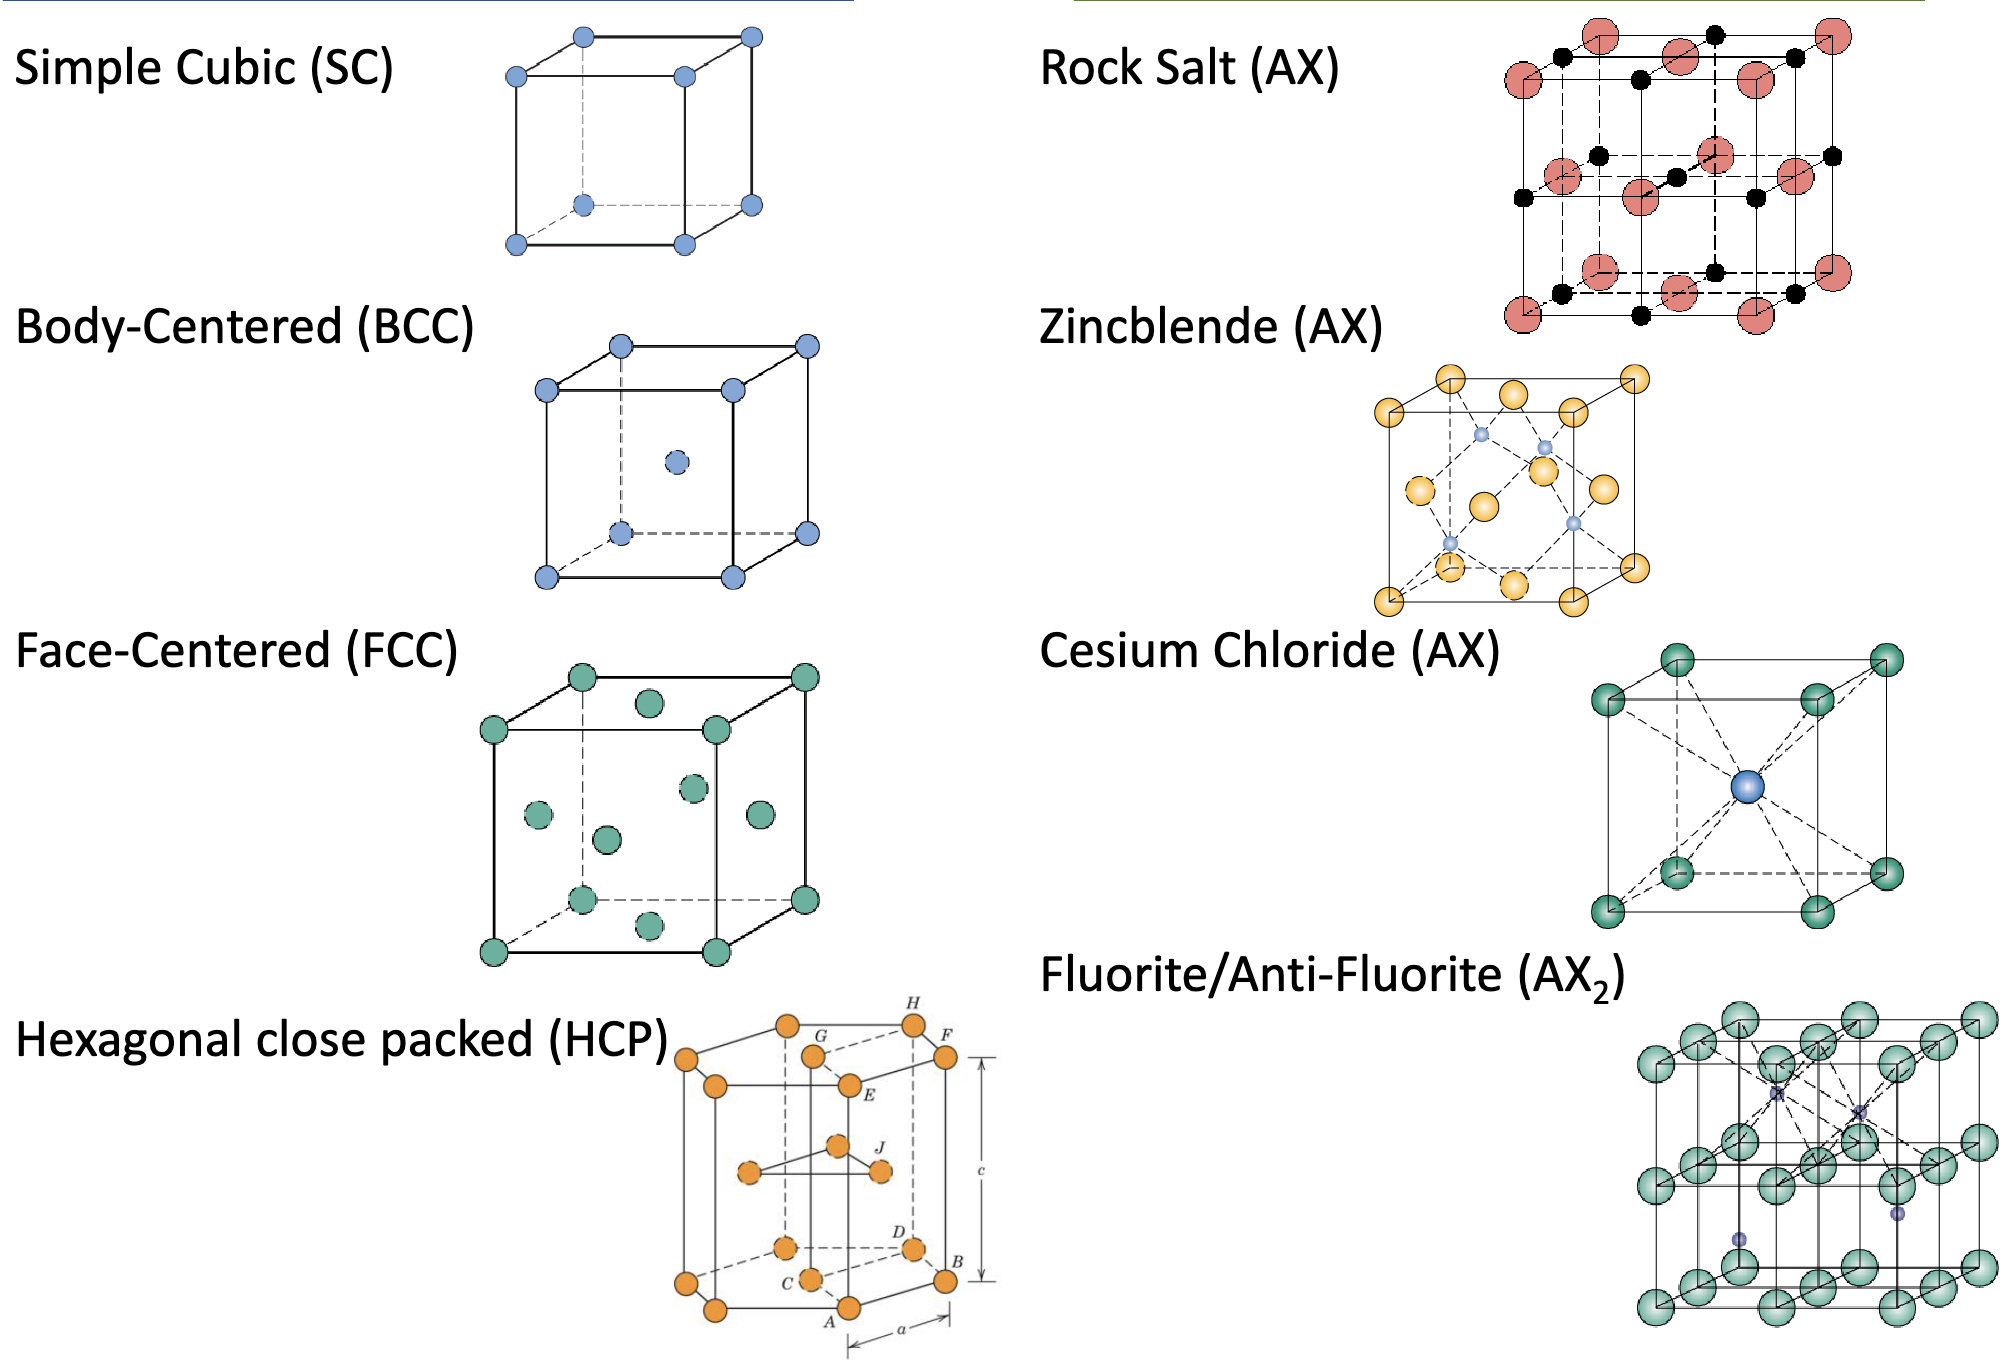
\includegraphics[width=0.8\textwidth]{structures.png}
\end{figure}

% area of equlateral triangle & special triangles



\begin{figure}[H]
    \centering
    \begin{minipage}{0.4\textwidth}
        \centering
        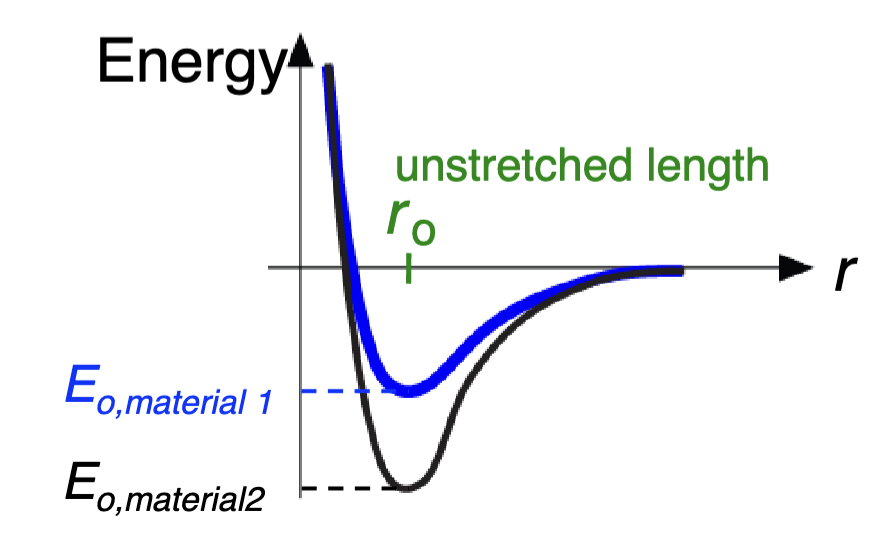
\includegraphics[width=\textwidth]{energy.png}
    \end{minipage}
    \hfill
    \begin{minipage}{0.4\textwidth}
        \centering
        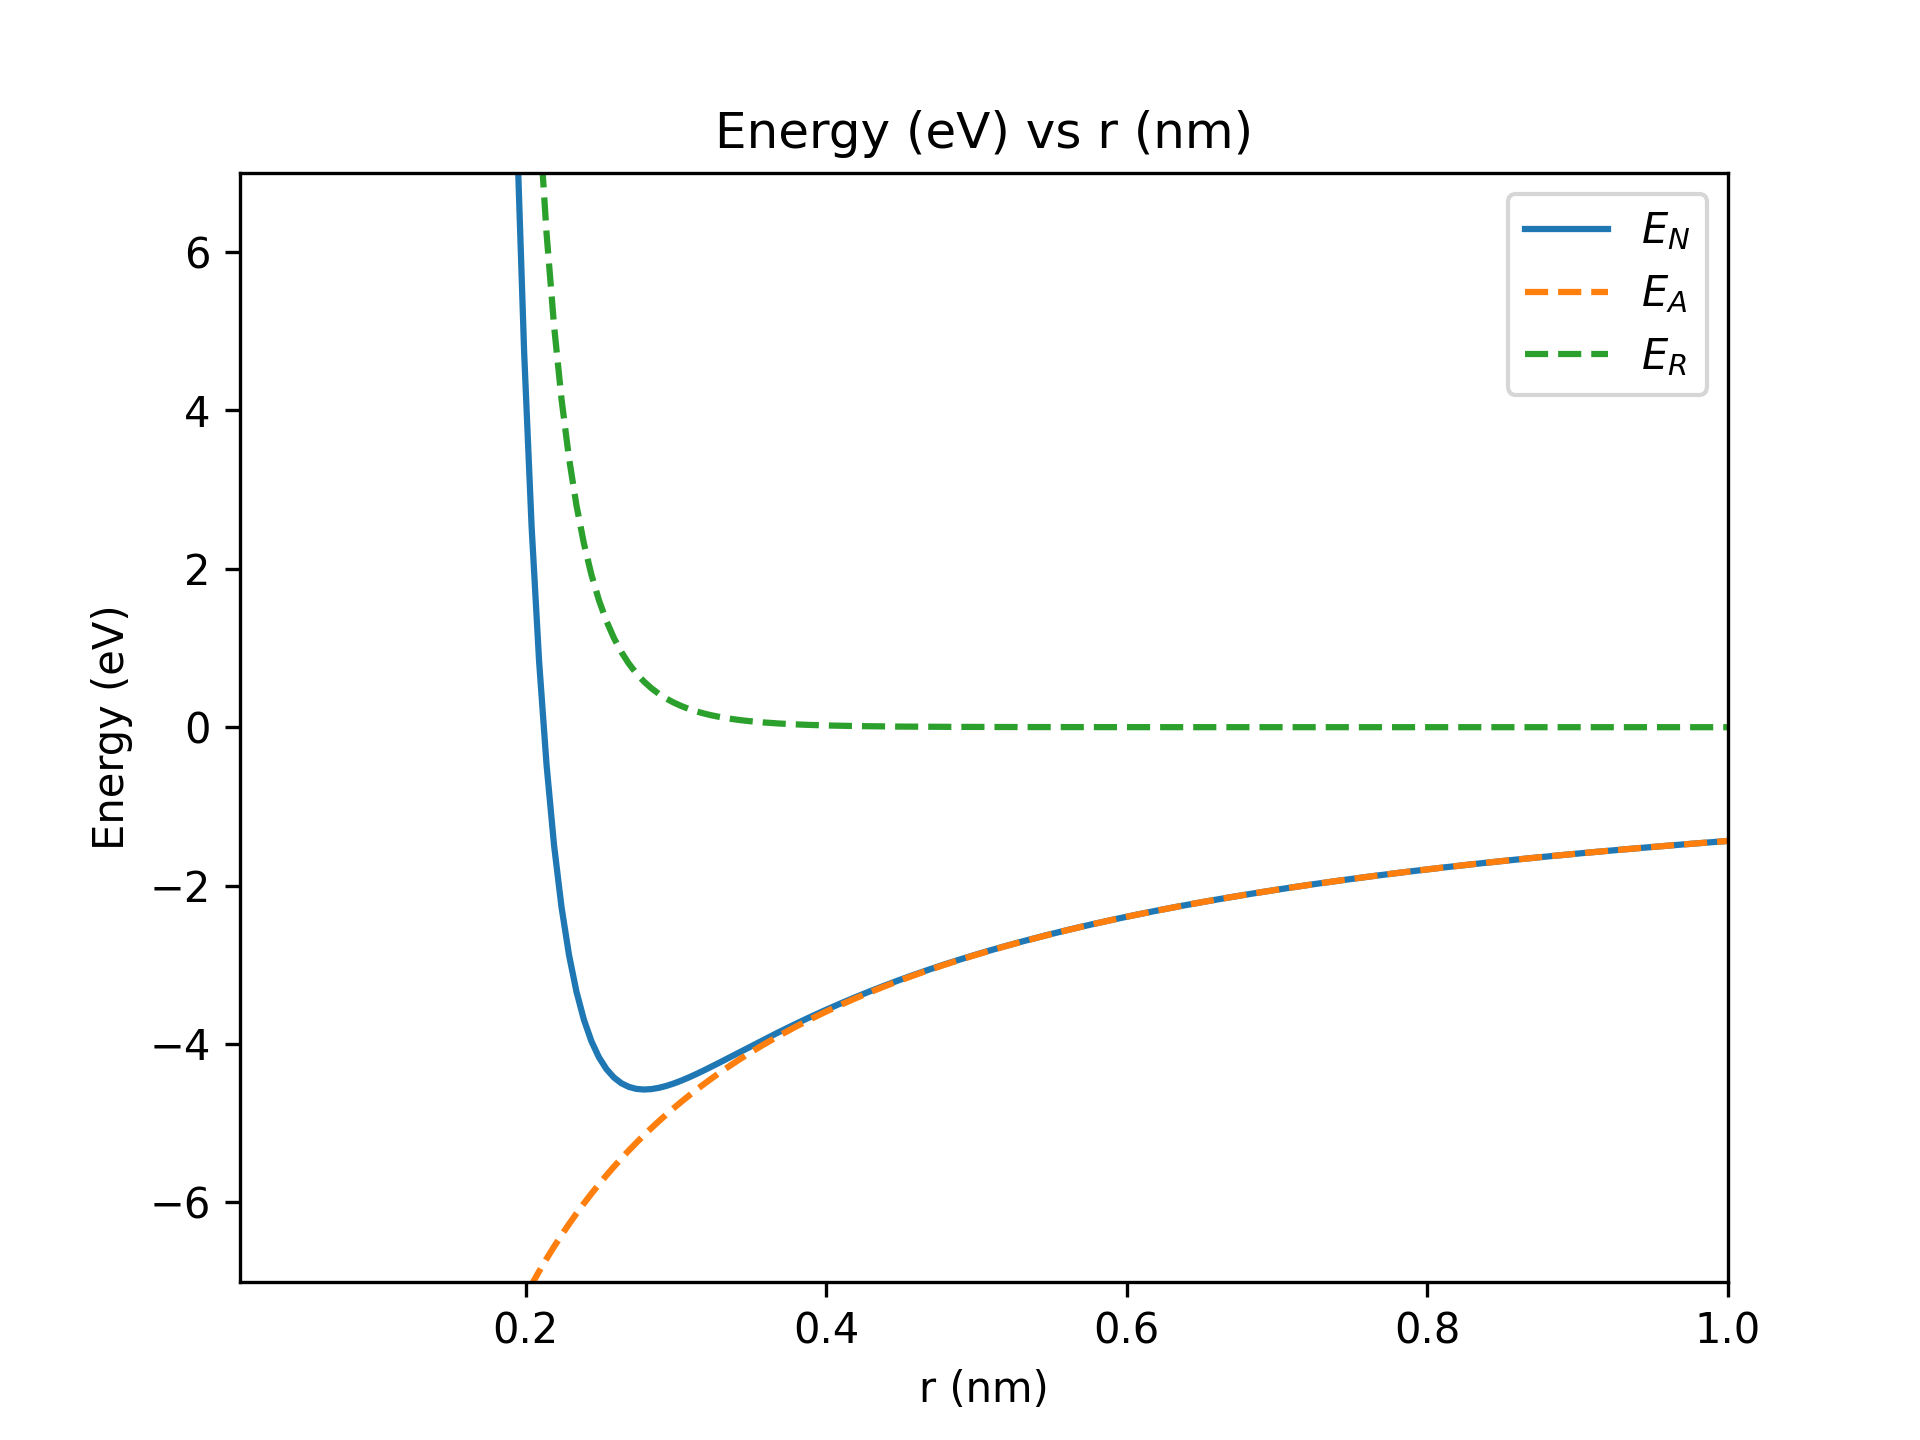
\includegraphics[width=\textwidth]{2a.png}
    \end{minipage}
    \hfill
    \begin{minipage}{0.2\textwidth}
        \centering
        \begin{tabular}{ c | c }
            Larger $E_0$ & Larger $T_m$ \\
            Smaller $E_0$ & Larger $\alpha$ \\
        \end{tabular}
    \end{minipage}
\end{figure}


\end{document}